Centrality metrics quantify the importance of nodes within a network based on link structures. PageRank \cite{rank-page99}, originally devised to rank web pages in search results, is one the most popular centrality metrics. It is based on the principle that pages receiving a greater number of high-quality links are of higher quality and, consequently, should be assigned higher ranks. Given the importance of such a metric, PageRank finds applications beyond web page ranking, including urban planning \cite{urban-zhang18}, traffic flow prediction \cite{traffic-kim15}, protein target identification \cite{banky2013equal}, evaluating the importance of brain regions \cite{zuo2012network}, identifying species crucial to environ\textit{mental} health \cite{allesina2009googling}, characterizing the properties of a software system \cite{chepelianskii2010towards}, and quantifying the scientific impact of researchers \cite{rank-senanayake15}. The growing availability of extensive interconnected / graph-based data has fueled substantial interest in parallel algorithms for computing PageRank \cite{rank-garg16, rank-nvgraph, rank-giri20, rank-guoqiang20, rank-li21, rank-sadi18, rank-sarma13}.\ignore{--- it has been implemented on multicore CPUs \cite{rank-garg16}, GPUs \cite{rank-nvgraph}, FPGAs \cite{rank-guoqiang20}, SpMV ASICs \cite{rank-sadi18}, CPU-GPU hybrids \cite{rank-giri20}, CPU-FPGA hybrids \cite{rank-li21}, and distributed systems \cite{rank-sarma13}.}

However, the dynamic nature of most real-world graphs, characterized by frequent edge insertions and deletions, poses challenges for recomputing PageRank from scratch, especially when dealing with small, rapid changes \cite{agarwal2012real, barros2021survey}. To address this, existing strategies instead iterate from ranks of vertices obtained in a previous snapshot of the graph, thereby reducing the required number of iterations for convergence. To further minimize the runtime needed, it is necessary to recompute only the ranks of vertices that are likely to change. One prevalent approach involves identifying reachable vertices from the updated regions of the graph and limiting processing to these vertices \cite{rank-desikan05, kim2015incremental, rank-giri20, sahu2022dynamic}. However, marking all reachable vertices as affected, even for minor rank changes, is likely to result in unnecessary computation. Further, updates may occur randomly, within dense graph regions --- necessitating processing a substantial portion of the graph. While our earlier work \cite{sahu2024incrementally} had addressed these issues on large dynamic graphs with uniformly random updates, we had observed that our proposed approach did not perform as well on real-world dynamic graphs --- parameter adjustment was needed to achieve acceptable performance. There is thus a need for a new approach that performs well on real-world dynamic graphs, where the nature of updates is different from a uniformly random update. In addition, to further improve performance, it is possible to halt rank updates for a vertex if its rank appears to have converged. This technical report introduces such an approach.




\subsection{Our Contributions}

This report introduces our Dynamic Frontier approach\footnote{\url{https://github.com/puzzlef/pagerank-openmp-dynamic}}, which, when given a batch update involving edge insertions and deletions, incrementally identifies affected vertices likely to undergo rank changes with minimal overhead. On a server equipped with a 64-core AMD EPYC-7742 processor, our Dynamic Frontier PageRank surpasses Static, Naive-dynamic, and Dynamic Traversal PageRank by $7.8\times$, $2.9\times$, and $3.9\times$ respectively, for uniformly random batch updates of size $10^{-7}|E|$ to $10^{-3}|E|$, where $|E|$ is the number of edges in the original graph. Additionally, our approach exhibits a performance improvement of $1.8\times$ for each doubling of threads. Additionally, our approach exhibits a performance improvement of $1.8\times$ for each doubling of threads.




%% - Use --- for a dash.
%% - Use ``camera-ready'' for quotes.
%% - Use {\itshape very} or \textit{very} for italicized text.
%% - Use \verb|acmart| or {\verb|acmart|} for mono-spaced text.
%% - Use \url{https://capitalizemytitle.com/} for URLs.
%% - Use {\bfseries Do not modify this document.} for important boldface details.
%% - Use \ref{fig:name} for referencing.

%% For a block of pre-formatted text: 
% \begin{verbatim}
%   \renewcommand{\shortauthors}{McCartney, et al.}
% \end{verbatim}

%% For a list of items:
% \begin{itemize}
% \item the ``ACM Reference Format'' text on the first page.
% \item the ``rights management'' text on the first page.
% \item the conference information in the page header(s).
% \end{itemize}

%% For a table:
% \begin{table}
%   \caption{Frequency of Special Characters}
%   \label{tab:freq}
%   \begin{tabular}{ccl}
%     \toprule
%     Non-English or Math&Frequency&Comments\\
%     \midrule
%     \O & 1 in 1,000& For Swedish names\\
%     $\pi$ & 1 in 5& Common in math\\
%     \$ & 4 in 5 & Used in business\\
%     $\Psi^2_1$ & 1 in 40,000& Unexplained usage\\
%   \bottomrule
% \end{tabular}
% \end{table}

%% For a full-width table:
% \begin{table*}
%   \caption{Some Typical Commands}
%   \label{tab:commands}
%   \begin{tabular}{ccl}
%     \toprule
%     Command &A Number & Comments\\
%     \midrule
%     \texttt{{\char'134}author} & 100& Author \\
%     \texttt{{\char'134}table}& 300 & For tables\\
%     \texttt{{\char'134}table*}& 400& For wider tables\\
%     \bottomrule
%   \end{tabular}
% \end{table*}


%% For inline math:
% \begin{math}
%   \lim_{n\rightarrow \infty}x=0
% \end{math},

%% For a numbered equation:
% \begin{equation}
%   \lim_{n\rightarrow \infty}x=0
% \end{equation}

%% For an unnumbered equation:
% \begin{displaymath}
%   \sum_{i=0}^{\infty} x + 1
% \end{displaymath}

%% For a figure:
% \begin{figure}[h]
%   \centering
%   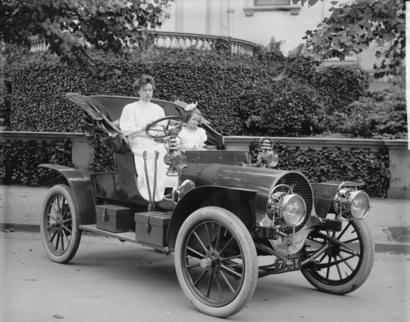
\includegraphics[width=\linewidth]{inc/sample-franklin}
%   \caption{1907 Franklin Model D roadster. Photograph by Harris \&
%     Ewing, Inc. [Public domain], via Wikimedia
%     Commons. (\url{https://goo.gl/VLCRBB}).}
%   \Description{A woman and a girl in white dresses sit in an open car.}
% \end{figure}

%% For a teaser figure.
% \begin{teaserfigure}
%   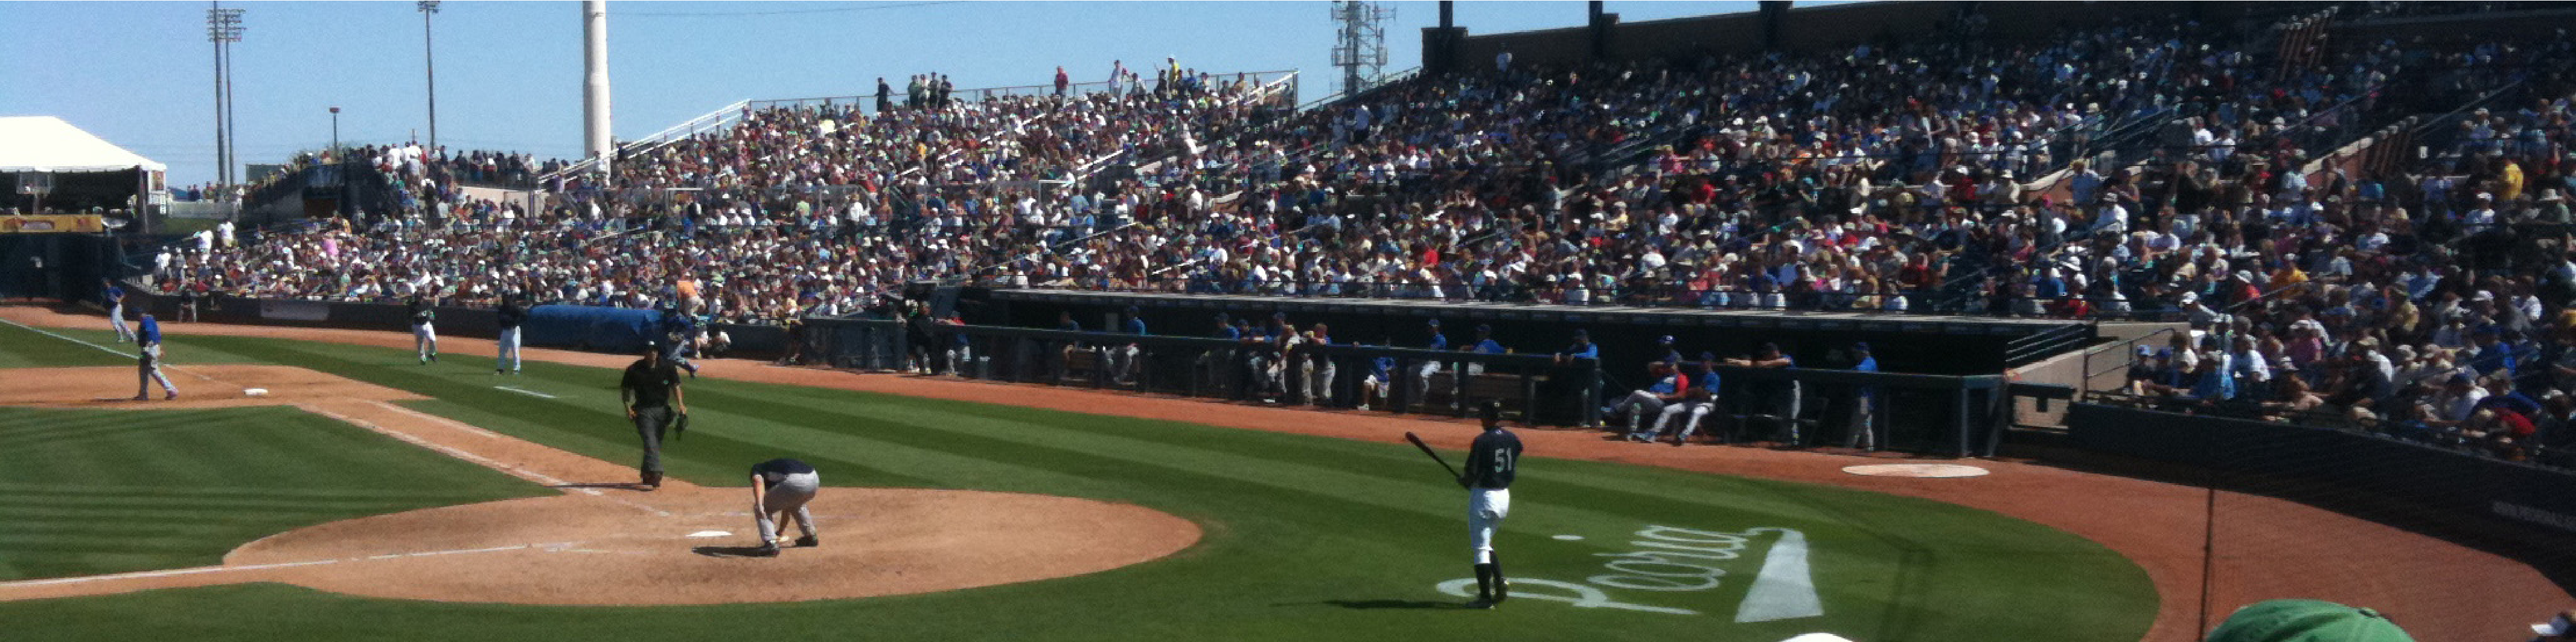
\includegraphics[width=\textwidth]{sampleteaser}
%   \caption{figure caption}
%   \Description{figure description}
% \end{teaserfigure}
